\chapter{Stato dell'arte e lavori correlati}
\label{sota}
In questo capitolo si discuteranno brevemente solo alcuni degli approcci più rilevanti al task di \textit{image layout classification}. Quello della composizione delle immagini non è un problema che viene spesso affrontato in ambito di ricerca, di conseguenza le risorse ad esso relative sono in numero limitato. Ciononostante, ci sono stati diversi tentativi nel corso degli anni di migliorare sempre più lo stato dell'arte.

\section{Prima del Deep Learning}
Prima di \cite{composition_dominant_geometric}, di cui si discuterà nella sezione successiva, non esistevano metodi automatici e affidabili per il task di classificazione della composizione, a causa della sua natura fortemente soggettiva e talvolta ambigua. Approcci precedenti si basavano solamente su un insieme limitato di aspetti della composizione, come il bilanciamento del peso visivo e la regola dei terzi, o sfruttavano procedure di clustering non supervisionato, senza però definire regole di composizione specifiche. In particolare, per riconoscere la RoT, alcuni metodi lavoravano localizzando il soggetto dell'immagine e calcolando la distanza fra il suo centroide e i punti di intersezione delle linee orizzontali con quelle verticali che formano la griglia (vedi Figura \ref{fig:rule_of_thirds}). 

Solamente \cite{fuzzy2012} ha provato a definire un metodo per categorizzare le regole di composizione in una più ampia varietà di classi, 8 in totale, considerando 25 criteri stabiliti sulla base di caratteristiche geometriche calcolate su ciascuna immagine. Questo approccio, però, è realizzato su un piccolo dataset di 80 fotografie e di conseguenza può produrre risultati inaffidabili su insiemi più ampi di immagini. Essendo regole costruite ad hoc per quel ridotto insieme di immagini, queste non possono coprire tutti i possibili casi di configurazioni presenti in un dataset più esteso. Inoltre, questo metodo non permette di classificare più classi di composizione all'interno della stessa immagine, o fatica nel farlo.

Altri approcci suddividono le foto in \textit{patches}, piccole regioni della stessa dimensione, e ne studiano poi il loro ordinamento all'interno dell'immagine e li utilizzano per localizzare soggetti localmente. Tecniche basate sulla valutazione di patches potrebbero però non tenere conto correttamente dei confini fra soggetti e ancora una volta faticano a valutare le immagini nel loro insieme.

Ci sono stati tentativi di suddividere le immagini tramite algoritmi di segmentazione e successivamente descrivere la composizione tramite le distribuzioni di colore o texture fra regioni, caratterizzandone la posizione nella foto, ma questo non basta a indurne la composizione globale.

\section{Fine-tuning di una CNN}
Il paper "\textit{Photographic composition classification and dominant geometric element detection for outdoor scenes}" \cite{composition_dominant_geometric} del 2017 è la prima istanza di uno studio completo e strutturato della classificazione della composizione delle immagini tramite \textit{deep learning}. 

Gli autori del paper utilizzano una CNN \textit{pre-trained} per imparare delle caratteristiche compositive discriminanti da un ampio insieme di immagini \textit{human-annotated}. L'architettura della rete utilizzata è esposta in Figura \ref{fig:arch_dominant_geometric}. L'allenamento preliminare della ResNet è fatto sul dataset ImageNet \cite{imagenet}, formato da 1000 classi, per evitare problemi di overfitting. Solo successivamente si fa un fine-tuning sul dataset KU-PCP, introdotto dal paper, e di cui si discuterà nel dettaglio nella Sezione \ref{kupcp}. KU-PCP diventerà di fatto il dataset standard per il task di image layout classification.

Il layer di \textit{softmax} prende in input solamente una classe alla volta da considerarsi come ground truth, quindi per affrontare il problema della classificazione multi-label, le immagini che possiedono classi multiple vengono fatte passare nella rete tante volte quante sono le classi di ground truth che possiedono.

La rete produce 9 \textit{confidence scores}, in numero pari alla molteplicità delle classi di composition nel dataset KU-PCP. Successivamente, ogni immagine viene categorizzata con la classe dallo score più alto. Nel caso ci sia un'altra classe che produce un punteggio superiore all'80\% di quello della più alta, allora anche questa viene considerata come risultato della classificazione.

\vspace{7mm}
\begin{figure}[hb]
    \centering
    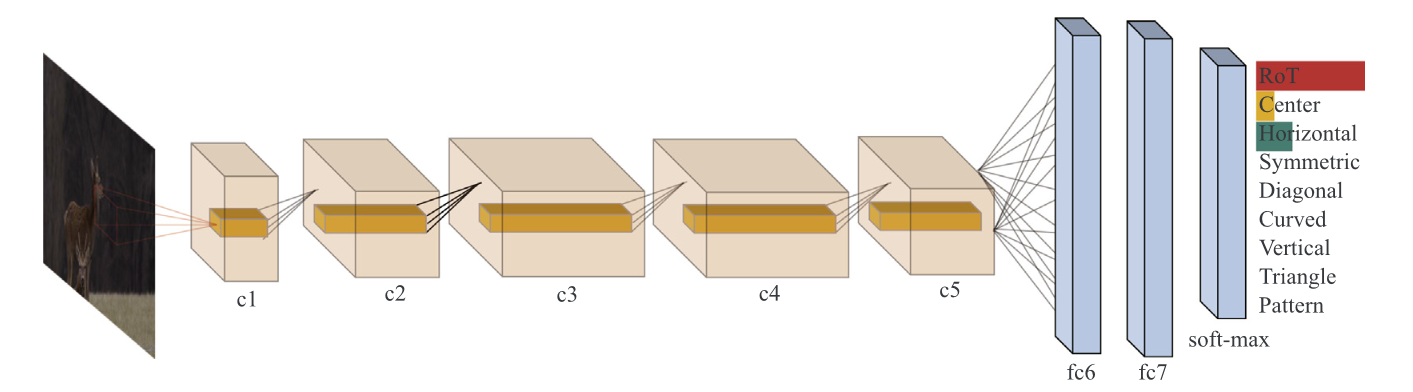
\includegraphics[height=40mm]{Immagini/sota/dominant_geometric_arch.png}
    \caption{L'architettura proposta da \cite{composition_dominant_geometric}, composta di cinque layer convoluzionali (c1, c2, c3, c4, c5) e tre \textit{fully connected layers} (fc6, fc7, soft-max). Il layer di soft-max produce i punteggi di confidenza per le 9 classi contenute nel dataset KU-PCP.}
    \label{fig:arch_dominant_geometric}
\end{figure}

\section{Spatial-invariant CNN}
\label{spatial-invariant-cnn}
Nel paper "\textit{\citefield{spatial_invariant_cnn}{title}}" \cite{spatial_invariant_cnn} si sostiene che il metodo precedentemente discusso sia indebolito dal fatto che il dataset KU-PCP contenga solamente fotografie professionali (uno dei suoi difetti, di cui si discuterà in Sezione \ref{lodb}), e che questo crei condizioni "troppo perfette" per il riconoscimento della composizione. Non si tiene conto delle \textit{snapshots}, fotografie scattate rapidamente, con uno smartphone, che possono presentare dei difetti come il non essere perfettamente allineate con l'orizzonte, o avere altre leggere imperfezioni, che caratterizzano la maggior parte delle fotografie che realizziamo nella vita quotidiana. Inoltre, gli autori sostengono che leggere variazioni spaziali, entro un determinato range, non influenzano la capacità di un umano di riconoscere la struttura compositiva dell'immagine (Figura \ref{fig:rotation_rstn}).

Viene proposta quindi una \textit{spatial-invariant} convolution neural network composta da una architettura denominata Rotation-Shift Transformer Network (RSTN) 

\begin{figure}[b]
    \centering
    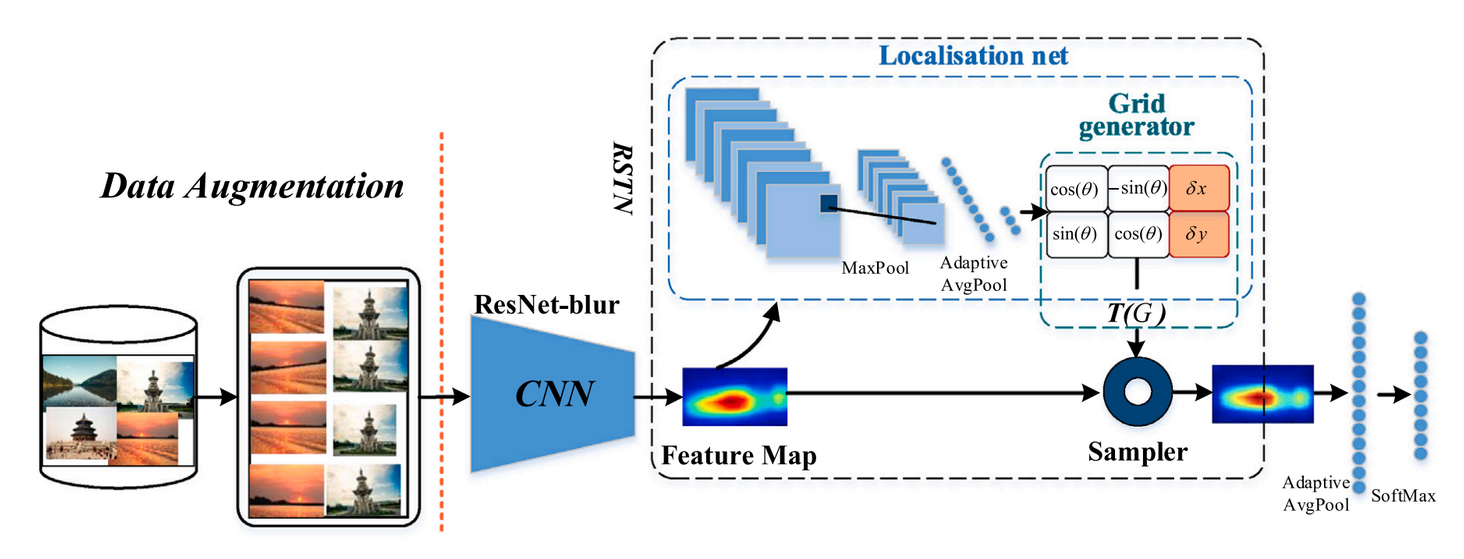
\includegraphics[height=50mm]{Immagini/sota/spatial_invariant_cnn.png}
    \captionsetup{justification=centering}
    \caption{Framework per la spatial-invariant convolution neural network.}
    \label{fig:rstn}
\end{figure}

Il processo di classificazione proposto è il seguente:
\begin{enumerate}
    \item \textbf{Augmentations}: a partire dalle immagini del dataset KU-PCP, si effettua una rotazione casuale nel range [-10, +10]°, che si è osservato non influire sulla percezione della composizione tanto da modificarne la tipologia riconosciuta dagli utenti.
    \item \textbf{Feature extraction}: si utilizza una ResNet pre-trained su ImageNet per estrarre una \textit{feature map} da utilizzare come descrittore dell'immagine in input nella parte di rete successiva, adibita al riconoscimento della distorsione applicata all'immagine.
    \item \textbf{Rotation Shift Transformer}: la sua struttura è ispirata dalle \textit{Spatial Transformer Networks} \cite{STN}. Si compone di:
    \begin{itemize}
        \item \textbf{Localization Net}: usa 2 layer convoluzionali e 2 fully connected layers per imparare tre parametri: l'angolo di rotazione \(\theta\) e i coefficienti di traslazione \(c, f\).
\item \textbf{Grid generator}: tramite i parametri prodotti dai layer convoluzionali precedenti, si può creare la matrice di trasformazione:
\[M = \begin{bmatrix}
\cos{\theta} & -\sin{\theta} & c \\
\sin{\theta} & \cos(\theta) & f \\
0 & 0 & 1
\end{bmatrix}\]
\item \textbf{Sampler}: effettuando il prodotto matriciale \(M \begin{pmatrix} x_i \\ y_i \\ 1 \end{pmatrix} \), dove \((x_i, y_i)\) sono le coordinate del pixel \(i\) nell'immagine augmentata, si può ricostruire l'immagine originale. In questo caso, la moltiplicazione viene fatta direttamente con i pixels della feature map prodotta dalla convoluzione della ResNet.
    \end{itemize}
\end{enumerate}
A questo punto si può passare la feature map ripristinata a un layer di pooling e un softmax, che produce i nove scores di confidenza per la classificazione della composizione.

Questo permette alla rete di imparare a trovare delle trasformazioni che possano correggere le piccole imperfezioni che caratterizzano foto non professionali, snapshots, e di conseguenza classificare le classi di composizione in maniera più robusta.

\begin{figure}[!ht]
    \centering
    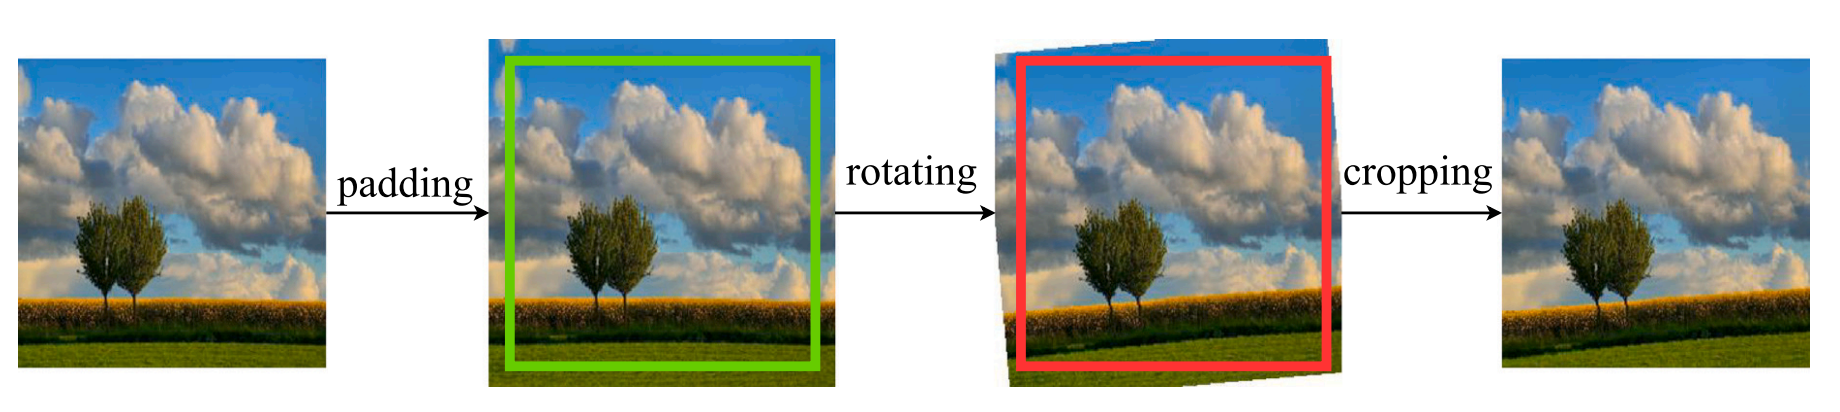
\includegraphics[height=30mm]{Immagini/sota/rotation_rstn.png}
    \caption{La rotazione dell'immagine viene effettuata introducendo del padding speculare intorno all'immagine, ruotando il risultato e croppando per tornare alle dimensioni originali. Gli autori osservano come, se la classe iniziale dell'immagine è quella di una leading line orizzontale data dall'orizzonte, distorcere l'immagine con una leggera rotazione non cambia il nostro giudizio sulla composizione, la percepiamo ancora come classe orizzontale riconoscendone il contesto.}
    \label{fig:rotation_rstn}
\end{figure}

\section{Grafi come descrittori del layout}
\label{graph}
Recentemente, nel marzo del 2024, è stato pubblicato il paper "\textit{\citefield{graph}{title}}" \cite{graph}. Gli autori sostengono che grandi problemi di approcci supervisionati nell'ambito della classificazione dell'image layout e task correlati siano il dipendere da datasets costosamente etichettati e la mancanza di adattabilità dei modelli nell'imparare le sfumature più fini della composizione. Per questo motivo si decide di cambiare completamente approccio, cioè di utilizzare la self-supervision, che non necessita di labels. 

La novità da Zhao et al. è quella di individuare nelle immagini delle primitive di base che incapsulino l'informazione di layout a diversi livelli, e di mapparle su una struttura a \textbf{grafo eterogeneo}. Dopodichè, si introduce un \textit{pretext task} ad hoc, in coppia con una funzione di loss apposita, progettati per poter permettere l'apprendimento autonomo. 
Con grafo eterogeneo si intende un grafo i cui archi e nodi possono appartenere a domini semantici diversi. I dettagli su self-supervision e pretext task verranno approfonditi nel prossimo capitolo. Stabiliti questi principi, gli autori introducono una architettura di rete in grado di comprimere questi grafi descrittori di ogni immagine in una rappresentazione vettoriale di dimensionalità ridotta, da usare poi per la classificazione.

Un altro importante contributo del paper in oggetto è l'introduzione del dataset \textbf{LODB} \cite{LODB}, costruito sulla base di KU-PCP e nato con l'obiettivo di compensare ai più grandi difetti di quest'ultimo. Presenta una più ampia gamma di categorie di layout (17 classi, contro le 9 di KU-PCP) e più semanticamente ricche. I dettagli verranno discussi nella Sezione \ref{lodb}.

\begin{figure}[!ht]
    \centering
    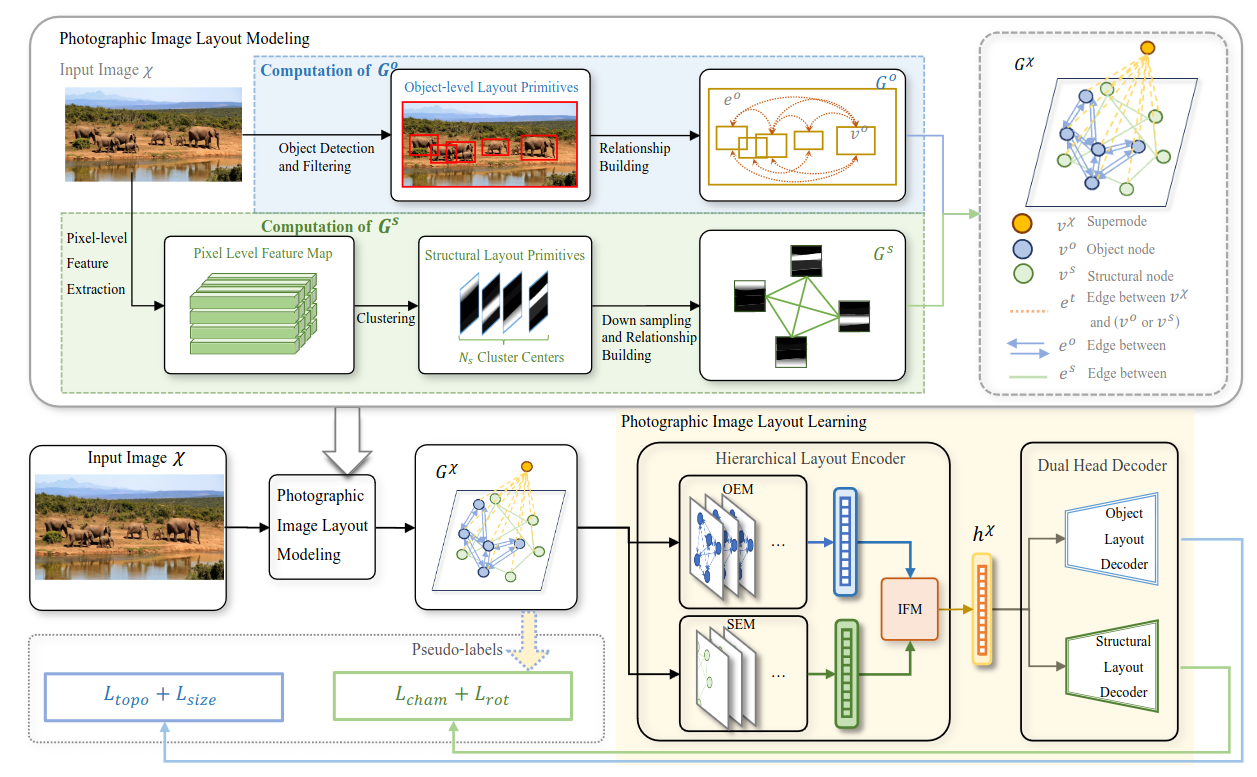
\includegraphics[width=\textwidth]{Immagini/sota/graph_arch.png}
    \caption{Workflow seguito da \cite{graph}.}
    \label{fig:arch_graph}
\end{figure}

Di seguito una breve spiegazione delle componenti del workflow. A partire da una immagine \(\chi\), i grafi coinvolti sono due:
\begin{itemize}
    \item Grafo \(G^s\), relativo alla struttura del layout. Secondo la teoria della Gestalt, primitive visivamente simili o in prossimità nell'immagine vengono percepite come un'unica entità. Per questo motivo, si utilizza una rete pre-allenata come feature extractor da ogni pixel dell'immagine e si fa del clustering sulle feature maps prodotte. Si costruisce il grafo \(G^s\) avente come nodi i clusters individuati, mentre come archi le relazioni di co-occorrenza fra nodi, cioè quanto spesso le primitive strutturali appaiono insieme o in vicinanza all'interno della foto.
    \item Grafo \(G^o\), relativo agli oggetti nell'immagine. Le immagini presentano generalmente uno o più oggetti salienti, che possono essere identificati tramite le rispettive \textit{bounding boxes}, le cui caratteristiche (dimensione, posizione) costituiranno i nodi del grafo. Gli archi codificano aspetti come le dimensioni relative fra due boxes, la distanza fra loro.
\end{itemize}

Senza scendere nei dettagli relativi alla funzione di loss utilizzata, si allena la rete in maniera self-supervised a imparare le caratteristiche di \(V^s\), l'insieme dei nodi del primo grafo, utilizzando come informazioni \(E^s\), gli archi dello stesso. Allo stesso modo, si introduce un secondo pretext task volto alla ricostruzione delle relazioni topologiche fra bounding boxes e i relativi centri, e un terzo task dedito ad effettuare regressione sulla dimensione delle boxes. Questo permette alla rete di imparare features molto più espressive dalle immagini che riceve, senza la necessità di labels, godendo di tutti i vantaggi che la self-supervision porta (approfondito in Capitolo \ref{ssl}). La procedura viene realizzata tramite un encoder costituito da una \textit{Graph Attention Network}, argomento che non è stato approfondito nel corso di questo stage. 

L'aspetto più importante da trarre da questo studio, oltre l'introduzione di LODB, è la nascita di metodi self-supervised volti alla classificazione della composizione, che sono in grado di imparare features espressive ad essa relative, e soprattutto in maniera autonoma. Questo rende ancora più rilevante un confronto coi metodi di self-supervised learning già stabiliti e di successo, come DINOv2. 